
\chapter{Návrh a implementácia}
\label{kap:implementacia}

V kapitole opisujeme priebeh vzniku aplikácie, implementačné detaily, postupy a rozhodnutia. Základné členenie obsahu je podľa modulov, za ktoré považujeme celky aplikácie ako editor kódu v grafickom jazyku, modul pre sériovú komunikáciu či modul pre simuláciu. Súčasťou sú tiež implementačne zmeny v riadiacom programe robota.

Vývoj začíname návrhom systému, ktorý umožní v aplikácii sprístupniť rôzne programovacie verzie pre rôzne modely robota a rôzne typy riadiaceho programu. Pokračujeme návrhom kostry a vizuálnej podoby aplikácie, v ktorej neskôr vzniknú jednotlivé moduly. V prvej fáze implementujeme časti podporujúce komunikáciu s aktuálnou verziou riadiaceho programu robota Otto a jeho programovanie. Nasleduje etapa rozširovania funkcionalít (hlavne grafického jazyka) a práca na module simulácie.

%K orientácii v štruktúre aplikácie môže byť nápomocný obrázok \ref{obr:app-structure}, kde sú v stĺpcoch znázornené jednotlivé moduly. Zobrazené sú tiež ich závislosti na technológiách a zdrojových súboroch.

%\begin{figure}
%\centerline{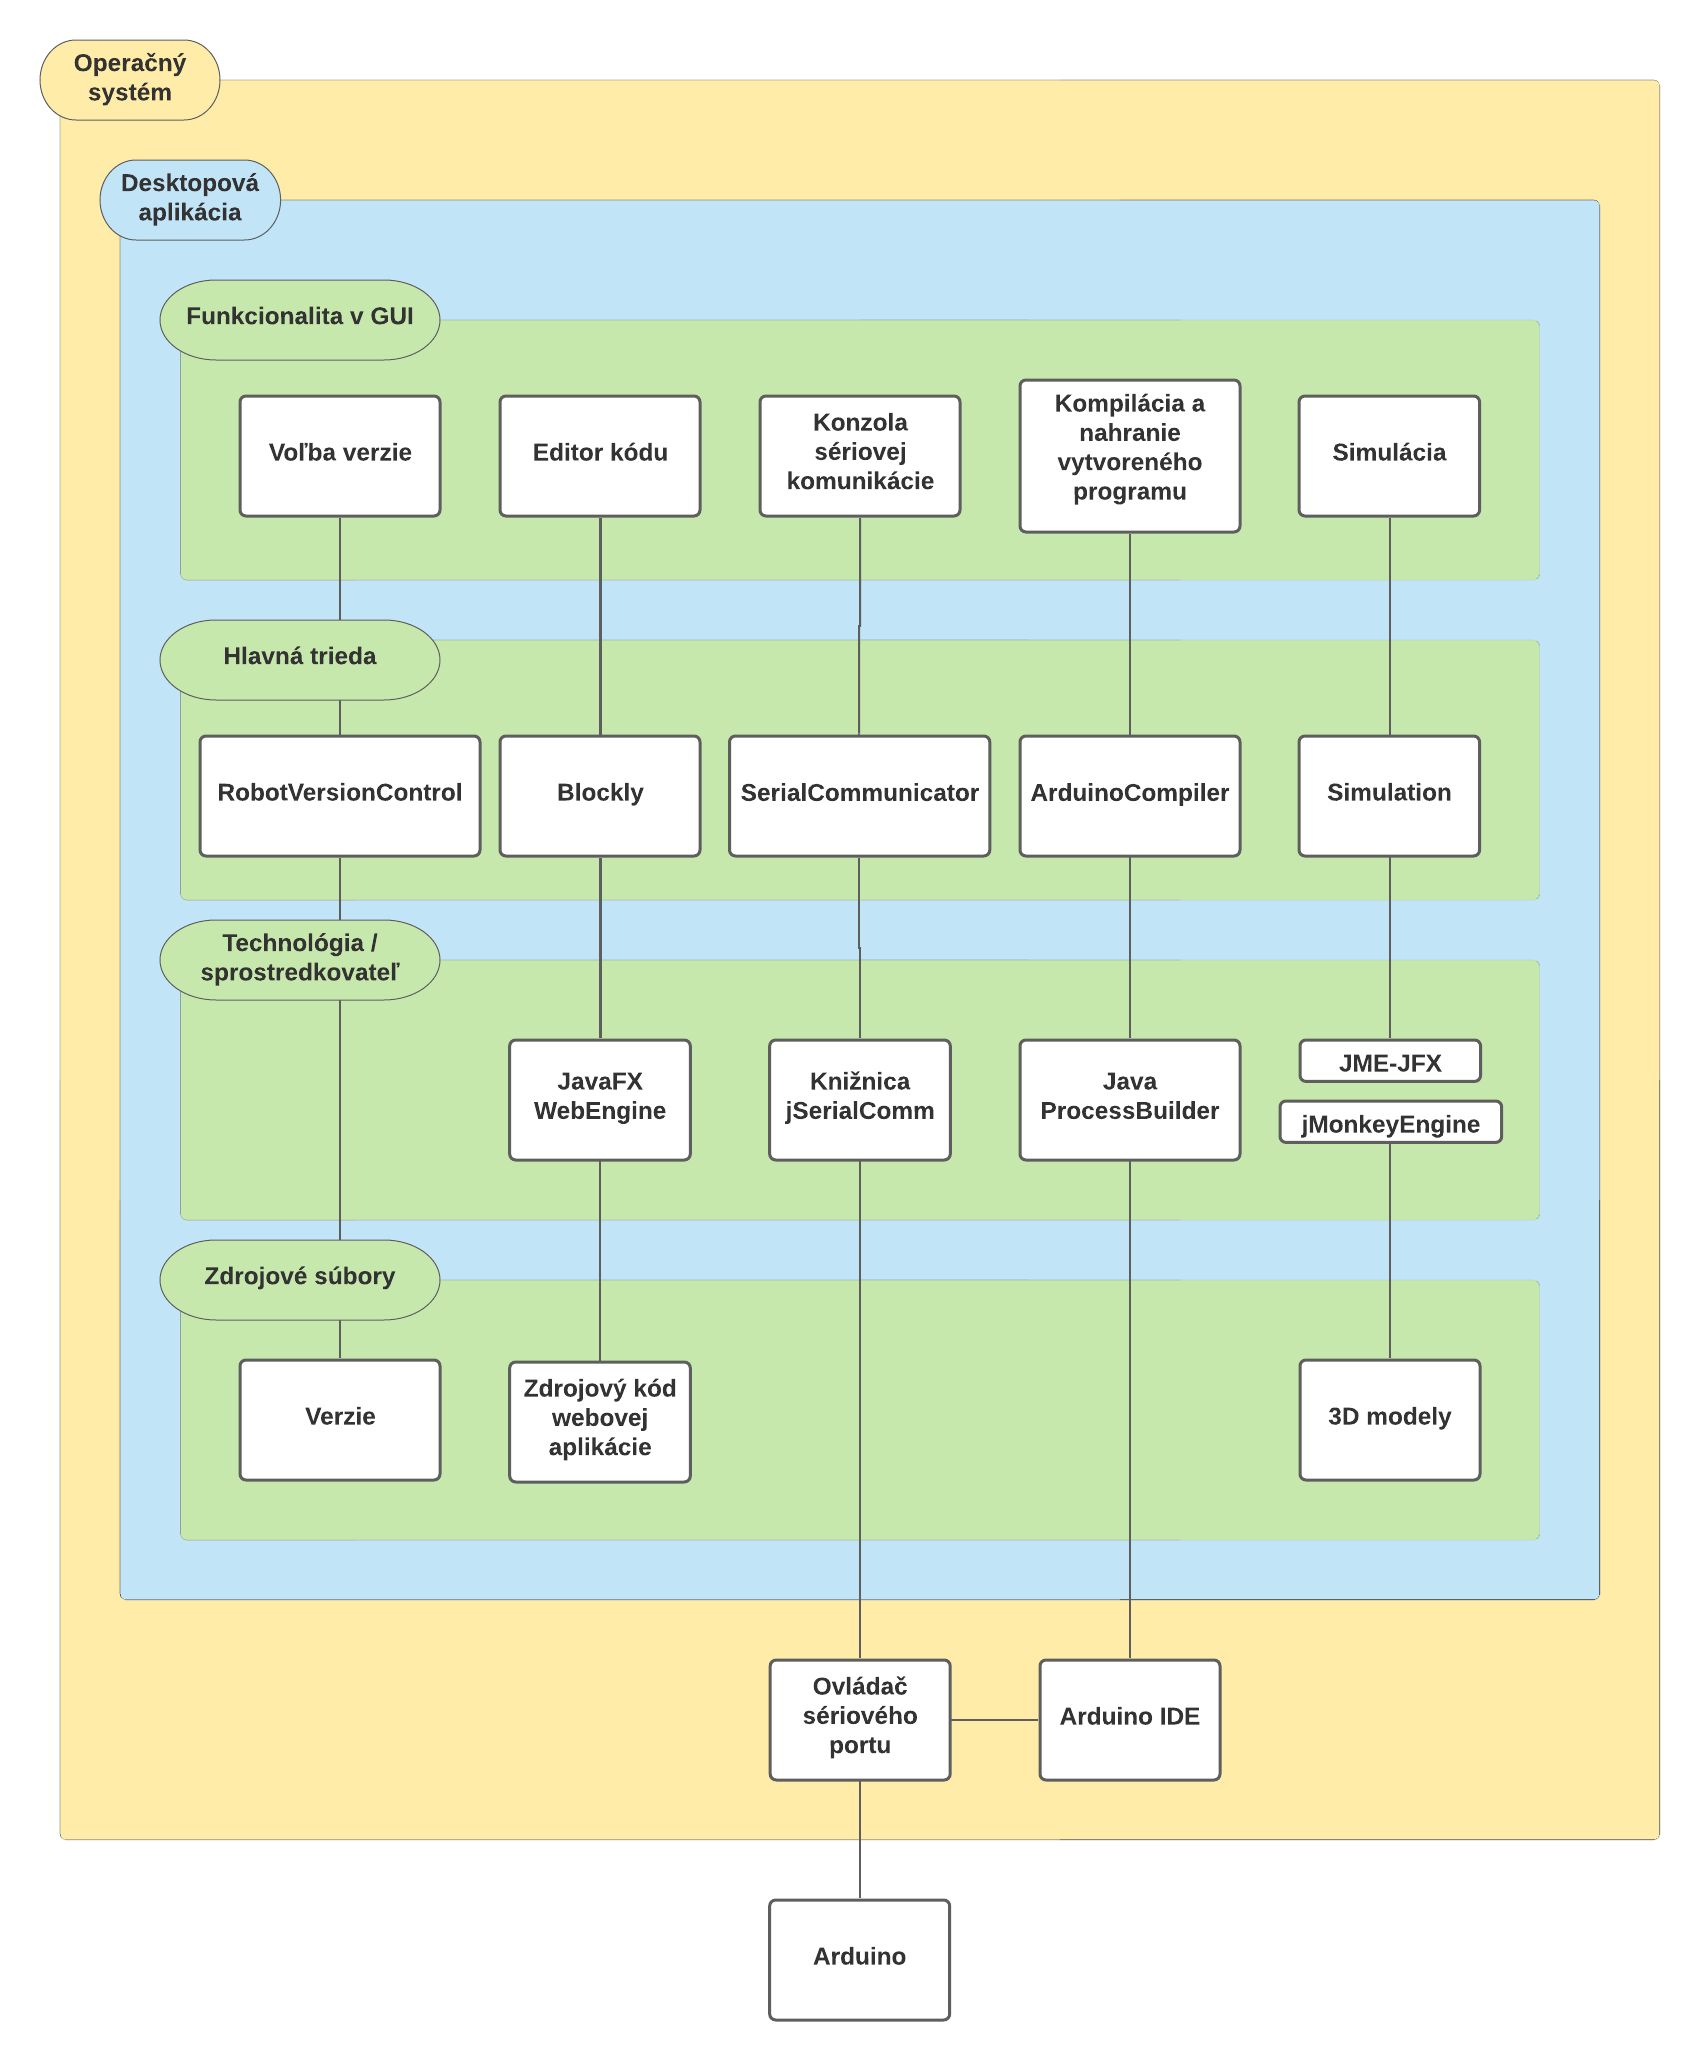
\includegraphics[width=1\textwidth]{images/app-structure}}
%\caption[Štruktúra aplikácie]{Štruktúra aplikácie}
%\label{obr:app-structure}
%\end{figure}


%%%%%
% %%% Modulárny systém verzií
%%%%%
\section{Systém verzií}
\label{sec:system-verzii}
Systém umožňuje definovať správanie jednotlivých modulov aplikácie (editor kódu, modul sériovej komunikácie, modul pre kompiláciu a nahranie riadiaceho programu, modul simulácie) pomocou konfiguračných súborov. Interakcia s aplikáciou začína vyhľadaním, výberom a načítaním takéhoto súboru --- verzie, ktorá určuje pre jednotlivé moduly ich počiatočnú konfiguráciu (nastavenie po načítaní konfiguračného súboru verzie, pred interakciou užívateľa s aplikáciou) a ich správanie počas interakcie s užívateľom (kým nie je načítaná iná verzia alebo ukončená aplikácia). Úlohou verzií je zabezpečiť nenáročnú rozšíriteľnosť a konfigurovateľnosť aplikácie parametrizáciou modulov. Počas tvorby aplikácie vznikli dve verzie, \uv{Otto 2020 Robotická liga} a \uv{Otto 2021 Procedural}.

\subsection{Obsah konfiguračného súboru verzie}
\label{sub:konfig-subor-verzie}
Súbor reprezentujúci verziu je tvorený množinou dvojíc kľúč--hodnota. Zoznam použitých kľúčov a význam priradenej hodnoty definuje nasledovná tabuľka.

\begin{table}\footnotesize
\centering
\begin{tabular}{ |p{3.8cm}|p{10cm}|  }
 \hline
	\multicolumn{2}{|c|}{\textbf{Všeobecné informácie o verzii}} \\
 \hline
	\textit{kľúč} & \textit{hodnota}\\
 \hline
	name&textový identifikátor verzie pre používateľa\\
	robotMaxMemory&číslo, limit pre súčet veľkostí vybraných logických modulov\\
	moduleCount&počet logických modulov\\
	exampleCount&počet ukážkových programov\\
 \hline

 \multicolumn{2}{c}{} \\
 \multicolumn{2}{c}{\textbf{Informácie pre modul editor kódu GPJ}} \\
 \hline
	\textit{kľúč} & \textit{hodnota}\\
 \hline
 	toolbox&XML definícia obsahu ponuky prvkov GPJ\\
 	workspace&XML definícia iniciálneho obsahu pracovnej plochy editora GPJ\\
 	categories&zoznam názvov kategórií v ponuke prvkov GPJ\\
 	generator&označenie generátora kódu (\uv{prekladača} GPJ)\\
 \hline

 \multicolumn{2}{c}{} \\
 \multicolumn{2}{c}{\textbf{Informácie pre modul kompilácie a modul sériovej komunikácie}} \\
 \hline
	\textit{kľúč} & \textit{hodnota}\\
 \hline
	programInRam&pravdivostná hodnota, určenie, či má byť pre použitie verzie nahraný do mikropočítača statický program\\
	programLocation&(voliteľné) relatívna cesta k statickému riadiacemu programu\\
	codeToConsole&pravdivostná hodnota, určenie, či preložený program z GPJ možno odostať priamo cez sériovú komunikáciu, bez kompilácie\\
 \hline

 \multicolumn{2}{c}{} \\
 \multicolumn{2}{c}{\textbf{Informácie pre modul načítania @ choreografie}} \\
 \hline
	\textit{kľúč} & \textit{hodnota}\\
 \hline
	codeLoader&označenie parsera pre vytvorenie prvkov GPJ z \textit{@ choreografie}\\
 \hline

 \multicolumn{2}{c}{} \\
 \multicolumn{2}{c}{\textbf{Zoznam logických modulov, pre modul X (kde X je celé číslo)}} \\
 \hline
	\textit{kľúč} & \textit{hodnota}\\
 \hline
	moduleX.name&názov, textový identifikátor pre používateľa\\
	moduleX.description&opis, textový identifikátor pre používateľa\\
	moduleX.required&pravdivostná hodnota, určenie, či je logický modul povinným\\
	&(ak áno, vždy je súčasťou výberu)\\
	moduleX.size&veľkosť kompilovaných súborov modulu\\
	moduleX.categories&zoznam názvov súvisiacich kategórií v ponuke prvkov GPJ modulu editor kódu\\
	moduleX.header&(voliteľné) označenie kompilovaného súboru, časť \textit{header}\\
	moduleX.setup&(voliteľné) označenie kompilovaného súboru, časť \textit{setup}\\
	moduleX.footer&(voliteľné) označenie kompilovaného súboru, časť \textit{footer}\\
 \hline

 \multicolumn{2}{c}{} \\
 \multicolumn{2}{c}{\textbf{Zoznam ukážkových programov, pre ukážku X (kde X je celé číslo)}} \\
 \hline
	\textit{kľúč} & \textit{hodnota}\\
 \hline
	exampleX.name&názov, textový identifikátor pre používateľa\\
	exampleX.description&opis, textový identifikátor pre používateľa\\
	exampleX.modules&zoznam poradových čísel použitých logických modulov\\
	exampleX.workspace&XML definícia (iniciálneho) obsahu pracovnej plochy editora GPJ\\
 \hline
\end{tabular}
\end{table}\normalsize

\subsection{Princíp}
Systém verzií sprístupní po spustení aplikácie používateľovi možnosť vyhľadať dostupné verzie. Po tomto procese môže byť verzia zvolená výberom zo zoznamu názvov verzií (hodnota priradená kľúču \textit{name}). Následne je podľa hodnoty \textit{programInRam} určené, či verzii prislúcha \uv{statický} riadiaci program mikropočítača.
	
Ak k verzii neprislúcha statický riadiaci program (hodnota \textit{programInRam} je záporná), nasleduje po voľbe verzie výber \textit{logických modulov}.
Jedná sa o (tematické) celky funkcionalít, určujú, ktoré prvky budú v editore GPJ k dispozícii a ktoré podporné súbory modulov (časti \textit{header, setup a footer}) riadiaceho programu budú kompilované. Používateľovi je pre tento účel zobrazené dialógové okno, pre každý modul zobrazuje názov, opis a veľkosť. Na základe informácie \textit{robotMaxMemory} je počet vybraných modulov limitovaný tak, aby súčet veľkostí vybraných modulov túto hodnotu nepresiahol. Logické moduly tiež umožňujú zjednodušiť programovanie začiatočníkom obmedzením množstva dostupných funkcií.

Ak k verzii prislúcha statický riadiaci program, je po jej zvolení zobrazená ponuka na jeho nahratie (modul kompilácie a nahratia kódu je spustený so vstupom definovaným parametrom \textit{programLocation} a následne je znefunkčnený, nakoľko kód vytváraný v GPJ tejto verzie nie kompilovateľný C++ kód). V tomto prípade nie je používateľovi umožnená voľba logických modulov, automaticky sú zvolené všetky dostupné.

Po voľbe logických modulov alebo nahraní statického riadiaceho programu nasleduje nastavenie ostatných modulov aplikácie. Pre modul editora GPJ je vo verzii uvedené, ktoré prvky GPJ majú byť k dispozícii. Obsah ponuky prvkov GPJ (obr.\ref{obr:gui-layout}, priestor A) je inicializovaný načítaním XML definície pod kľúčom \textit{toolbox}. Na základe voľby logických modulov sú potom zobrazené len kategórie (komponenty XML), ktorých názvy sú súčasťou zoznamu názvov kategórií niektorého z vybraných logických modulov (kľúč \textit{moduleX.categories}). Ostatné kategórie zo zoznamu (zoznam pod kľúčom \textit{categories}) sú skryté. Pre modul editora GPJ je vo verzii tiež definované počiatočné rozmiestnenie prvkov GPJ v editore (XML reprezentácia obsahu pod kľúčom \textit{workspace}), ktoré používateľ následne upravuje a určenie generátora (pod kľúčom \textit{generator}) (kapitola \ref{sec:editor-kodu}), ktorý sa použije pri preklade GPJ.

V module sériovej komunikácie je na základe hodnoty \textit{codeToConsole} umožnené alebo znefunkčnené priame odoslanie generovaného kódu cez pripojený sériový port.

Modul kompilácie je po voľbe logických modulov konfigurovaný na základe hodnôt \textit{moduleX.header}, \textit{moduleX.setup} a \textit{moduleX.footer} zvolených modulov. K logickému modulu môžu prislúchať súbory definujúce podporne funkcie (v jazyku C++), ktorých volania sú súčasťou prekladu prvkov GPJ sprístupnených daným logickým modulom. Na základe voľby logických modulov je vytvorený zoznam takýchto súborov, ktoré pri kompilácií spracuje modul kompilácie (kapitola \ref{sub:arduinoIDE}).

Súčasťou definície verzie je tiež informácia, či je možné vygenerovať obsah editora GPJ z užívateľom vloženého kódu vo formáte trojíc celých čísel, reprezentujúcich choreografiu robota Otto (kľúč \textit{codeLoader}).

K verzii môžu byť tiež priložené definície ukážkových programov. Definujú prednastavené rozloženie prvkov v editore GPJ, ktoré možno načítať a ďalej upravovať. Nevyhnutné je pre každý ukážkový program definovať zoznam použitých modulov, aby bolo možné nastaviť kompilátor a kategórie prvkov GPJ zobrazené v editore.

\subsection{Verzia Otto 2020 Robotická liga}
\label{sub:verzia-otto-2020-rl}
Verzia predstavuje konfiguráciu aplikácie, v ktorej je možné tvoriť kód pre robota Otto ako trojice celých čísel (spôsob vyvinutý pre účely denných táborov, kapitola \ref{subsub:otto-programovanie}). Tento prístup vyžaduje, aby bol v Arduino nahraný \uv{statický} riadiaci program, ktorý následne interpretuje znaky prijaté cez sériovú komunikáciu. Vo verzii je teda definované, že pre jej použitie je nutné do robota nahrať takýto program a používateľ je po jej voľbe vyzvaný, aby tak učinil. Modul kompilácie je následne (na základe informácie vo verzii) znefunkčnený, nakoľko ďalšie programovanie robota prebieha priamym odosielaním znakov cez sériovú linku (kapitola \ref{subsub:otto-programovanie}).

Vo verzii \textit{Otto 2020 Robotická liga} sú v editore GPJ k dispozícii len prvky prezentovateľné trojicami celých čísel, ktorými je tvorená choreografia a prvky na obsluhu senzorov sú skryté, nakoľko tie riadiaci program nepodporuje. Generátor pre verziu \textit{Otto 2020 Robotická liga} prekladá prvky GPJ na trojice celých čísel.

\subsection{Verzia Otto 2021 Procedural}
\label{sub:verzia-otto-2021-procedural}
Verzia \uv{Otto 2021 Procedural} predstavuje konfiguráciu aplikácie, v ktorej je možné tvoriť kód pre robota Otto prvkami GPJ reprezentujúcimi prvky jazyka Arduino (C++). Po načítaní tejto verzie je užívateľovi umožnená voľba \textit{logických modulov}, ktoré sú vo verzii definované. Príkladom je logický modul \textit{senzory}, ktorý po výbere používateľovi sprístupní v GPJ bloky umožňujúce čítať aktuálne merané hodnoty alebo čakať na nameranie konkrétnej hodnoty. Možnosť odoslať kód vytvorený prekladom GPJ prostredníctvom sériovej komunikacie je znefunkčnená, namiesto toho je k dispozícii možnosť  kód kompilovať a vzniknutý riadiaci program odoslať do riadiacej jednotky robota použitím modulu kompilácie (kapitola \ref{sub:arduinoIDE}).

\newpage

%%%%%
% %%%    GUI
%%%%%
\section{Grafické rozhranie}
GUI aplikácie tvoríme pomocou JavaFX. Cieľom je vytvoriť prehľadné prostredie, v ktorom sa ľahko zorientuje i požívateľ nižšieho veku. Pri rozmiestňovaní jednotlivých prvkov sú nám nápomocné existujúce aplikácie, no zohľadňujeme i rady autorov knižnice Blockly \cite{blocklyBestPractices}, keďže komponent umožňujúci prostredníctvom nej programovať robota je v našej aplikácii dominantným. Z odporúčaní je zrejmé, že plochu pre manipuláciu s prvkami grafického jazyka je žiaduce maximalizovať a neoddeľovať ju od komponentu umožňujúceho tvorbu blokov (prvkov jazyka).

Ďalšie prvky vyžadujúce v aplikácii väčšiu plochu sú najmä výstupné, predovšetkým ide o výstup pre modul simulácie a výstup \uv{prekladača} grafického jazyka na kód následne kompilovaný a odosielaný do riadiacej jednotky robota. Taktiež je nutné zakomponovať do GUI modul pre komunikáciu s robotom, konzolu sériovej komunikácie.

Výsledné rozloženie môžete vidieť na obrázku \ref{obr:gui-layout}. Tvoriť kód v grafickom jazyku možno v časti \textit{A}, umožňujúcej výber blokov, a ich následným umiestňovaním v priestore \textit{B}. Sektor \textit{C} je vyhradený pre výstup modulu simulácie. Časť \textit{D} je zdieľaná modulom sériovej komunikácie a modulom umožňujúcim náhľad do kódu generovaného prekladom grafického jazyka, medzi ktorými možno prepínať. Nad spomínanými oblasťami sa nachádza lišta nástrojov, sprístupňujúcich funkcie ako vyhľadanie a pripojenie sériovej komunikácie či voľbu verzie programovaného riadiaceho programu robota.

\begin{figure}
\centerline{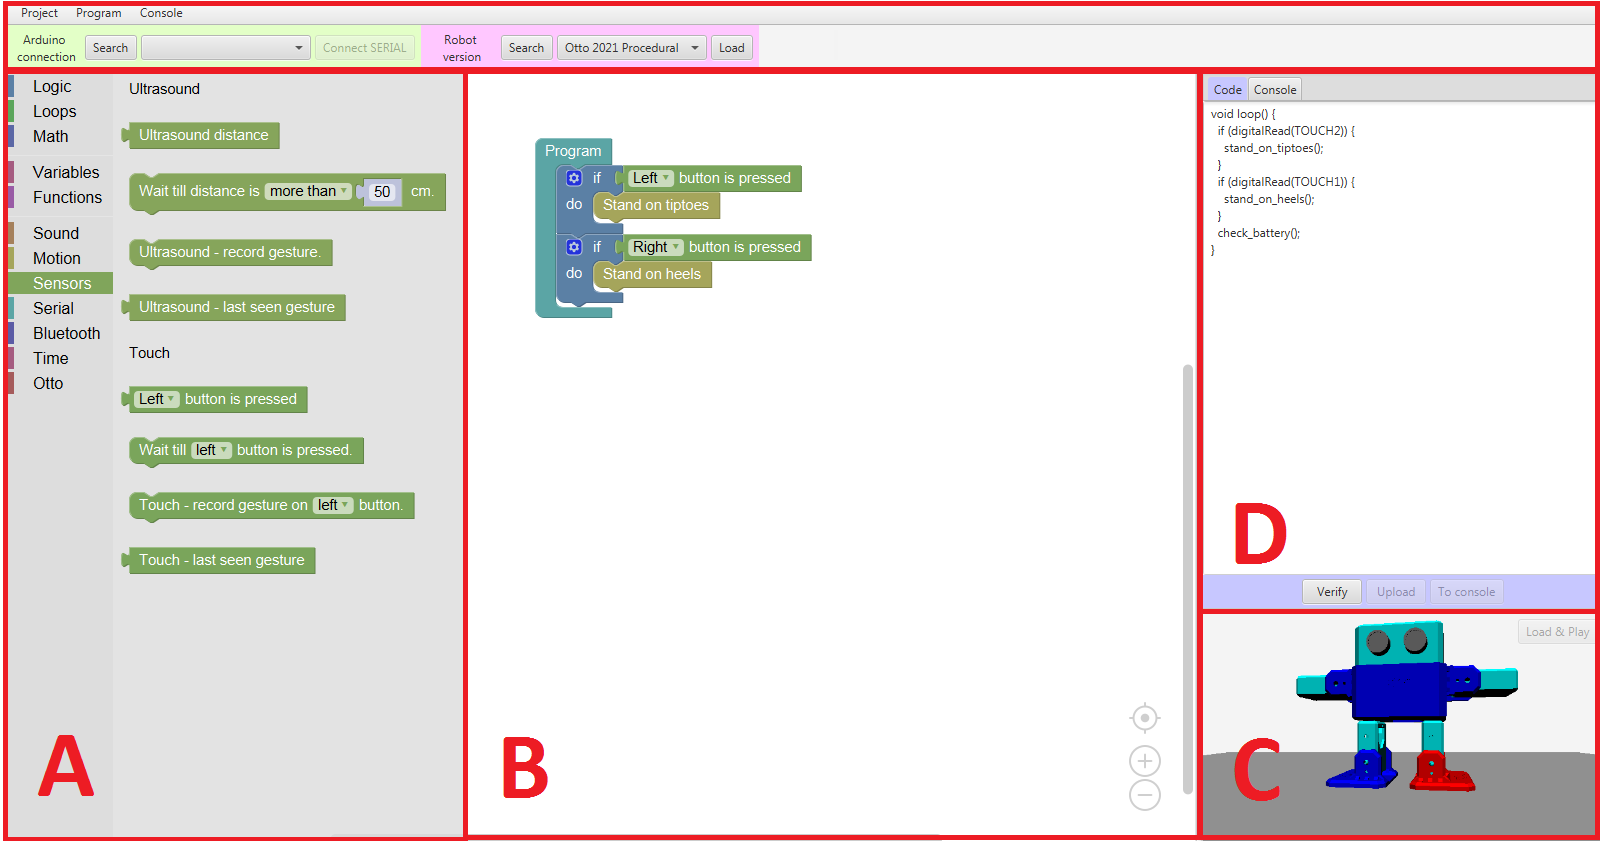
\includegraphics[width=1\textwidth]{images/rozlozenie-gui}}
\caption[Rozloženie používateľského rozhrania]{Rozloženie používateľského rozhrania}
\label{obr:gui-layout}
\end{figure}


%%%%%
% %%% Editor kódu
%%%%%
\section{Editor kódu}
\label{sec:editor-kodu}
Modul umožňujúci tvorbu (riadiaceho) programu pomocou grafického programovacieho jazyka (GPJ) je v podstate samostatnou webovou JavaScript aplikáciou. V GUI našej aplikácie je zobrazený jej výstup tvorený knižnicou Blockly v komponente WebView (webový prehliadač). Interakcia medzi vonkajšou Java aplikáciou a vnorenou JavaScript aplikáciou prebieha v Java pomocou inštancie WebEngine. Editor sa navonok skladá z dvoch hlavných častí --- ponuky prvkov GPJ (obr.\ref{obr:gui-layout}, priestor A), z ktorej používateľ vyberá požadované \uv{diely} GPJ a pracovnej plochy (obr.\ref{obr:gui-layout}, priestor B), v ktorej sú vybrané komponenty GPJ používateľom umiestňované, je nimi tvorený kód.

Konfiguráciu modulu editora kódu zabezpečuje systém verzií (kapitola \ref{sec:system-verzii}), ktorý využíva rozhranie poskytnuté knižnicou Blocky pre úpravu momentálne zobrazeného obsahu pracovnej plochy a ponuky prvkov GPJ. Obsah a rozloženie oboch týchto častí možno určiť načítaním ich definície vo formáte XML (súčasť verzií,  kapitola \ref{sub:konfig-subor-verzie}).

Rozhranie definuje i funkcie, ktorými je možné volať generátory GPJ. Ich úlohou je preklad prvkov GPJ na kód riadiaceho programu (prípadne jeho časti), ktorý je následne spracovávaný Java aplikáciou a kompilátorom. Usporiadaním v editore kódu sú použité bloky GPJ organizované v grafovej štruktúre, generátor je funkcia, ktorej parametrom je blok. Má prístup k poliam bloku (polia sú prvky pre výber možností, prípadne textový alebo číselný vstup. Zároveň má generátor prístup k vnoreným blokom (napríklad blok cyklu while má prístup k blokom v tele cyklu) a pripojeným \uv{nasledovníkom} --- bloku pod ním. Návratovou hodnotou je vhodne spracovaný kód so zakomponovaným obsahom potomkov a polí. Kód je generovaný rekurzívne, zvyčajne začínajúc na najvyššom bloku umiestnenom v editore.

Rozhranie tiež umožnuje získať aktuálny obsah pracovnej plochy zapísaný v XML reprezentácii a naopak, obnoviť obsah pracovnej plochy z poskytnutej XML reprezentácie. Tento mechanizmus využívame pre načítanie iniciálneho stavu pracovnej plochy (po voľbe a načítaní verzie) ale i načítanie ukážkových programov. Samozrejmosťou je implementácia funkcie umožňujúcej uloženie a znovu načítanie celého projektu.

Detailom implementácie prvkov a logiky vzniknutého grafického programovacieho jazyka je venovaná kapitola \ref{kap:navrh-gpj}.

\newpage

%%%%%
% %%%    Komunikácia, serial
%%%%%
\section{Komunikácia s robotom}
Možnosť komunikácie s robotom je jednou zo základných požiadaviek na našu aplikáciu. Umožňuje vyššiu interakciu s používateľom a je tiež nápomocná pri ladení programov (pomocné výpisy). Komunikácia s robotom na úrovni nahratia kompilovaného programu je predmetom časti \ref{sub:arduinoIDE}, tu je opísaná sériová komunikácia už bežiaceho programu v mikropočítači Arduino s našou aplikáciou. Jedná sa o komplementárnu časť systému k časti implementovanej v mikropočítači (sekcia \ref{sub:arduino}).

%\subsubsection{Komunikácia zo strany aplikácie}
V aplikácii je cieľom vytvoriť integrovaný terminál pre sériovú komunikáciu. Mikropočítač Arduino komunikuje po pripojení rozhraním USB a nainštalovaní príslušného ovládača v počítači s OS, ktorý nám toto spojenie sprostredkuje. Podobne pracuje i terminál v Arduino IDE (oficiálne IDE pre vývoj riadiacich programov Arduino) alebo program Putty (klient pre ssh, Telnet, Rlogin a sériovú komunikáciu \cite{putty}). Autori mikropočítača odporúčajú pre implementáciu sériovej komunikácie v Java použitie knižníc \cite{arduinoAndJava}. V článku o prepojení Java --- Arduino sú spomínané dve, údajne nespoľahlivá knižnica RXTX a možná alternatíva, knižnica jSerialComm, ktorú použijeme. 

jSerialComm je platformovo nezávislá knižnica, ľahko integrovateľná do našej aplikácie \cite{jSerialComm}. Umožňuje vyhľadávať pripojené dostupné sériové porty, ako aj obojsmernú komunikáciu po pripojení. Podporuje niekoľko typov operácie, v závislosti na blokovaní čítania z (zápisu do) sériového portu. V prípade čítania sú na výber alternatívy ako \textit{neblokovaná komunikácia}, v ktorej možno príkazom \textit{read()} skúsiť načítať dáta, ak však nie sú k dispozícii (neboli prijaté), vrátený je prázdny reťazec. Inou možnosťou je vynútenie čakania na možný príchod správy a to buď len po nejaký čas alebo až do jej prijatia. Vo oboch týchto prípadoch by ale v našej aplikácii bolo nutné cyklicky kontrolovať, či nejaké dáta nie sú k dispozícii (ako v mikropočítači), knižnica ale poskytuje vhodnejší prístup, registráciu callback funkcie. Tú knižnica zavolá po každom výskyte špecifikovanej udalosti, ktorou môže byť dostupnosť dát alebo prijatie ucelenej správy. V implementácii volíme možnosť volania callback funkcie po prijatí ucelenej správy, pričom za koniec správy je považovaný znak konca riadku (\textbackslash n --- line feed). Registrovaná callback funkcia správu načíta a zobrazí v termináli používateľovi.

Odosielanie správ je rovnako možné nastaviť do blokujúceho režimu, kde pri pokuse o zápis do sériového portu knižnica čaká buď to určitý čas alebo kým sa podarí odoslať požadovaný počet bajtov. Pre implementáciu volíme neblokovaný prístup, ak používateľ odošle dáta, sú zapísané hneď ako je to možné. Neblokovaný prístup umožní odoslanie viacerých správ, ktoré následne v rovnakom poradí knižnica odvysiela. Implementujeme tiež možnosť odosielať správy pozostávajúce z jedného znaku ihneď po stlačení požadovaného klávesu, bez nutnosti dodatočného potvrdenia odoslania. Táto funkcionalita je vhodná napríklad pri interakcii s robotom Otto v režime priameho riadenia (kapitola \ref{sub:otto}).


%%%%%
% %%%    Kompilácia, upload, Arduino IDE
%%%%%
\section{Kompilácia a nahranie riadiaceho programu}
\label{sub:arduinoIDE}
Kompiláciu a nahranie riadiaceho programu pri vývoji programov pre Arduino zvyčajne zabezpečuje Arduino IDE s grafickým používateľským rozhraním (sekcia \ref{sub:arduino}). Nahrávanie kompilovaného programu prebieha sériovou komunikáciou medzi Arduino IDE a bootloader programom v mikropočítači, zodpovednom za uloženie prijatého kódu do flash pamäte \cite{sketchUpload}. Overenie prenosu je uskutočnené spätným odoslaním celého programu z mikropočítača do IDE. Bootloader je spustený len určitý (krátky) čas po resetovaní procesora, ak v tomto časovom okne nie je zaznamenané nahrávanie riadiaceho programu, spustí sa posledný nahraný program. Procesor je resetovaný po obnove napájania ale i pri nadviazaní nového sériového spojenia.

Proces kompilácie a nahrania riadiaceho programu je možné implementovať na nižšej úrovni, samostatným volaním kompilátora a následným použitím knižnice jSerialComm pre nahranie a spätnú verifikáciu. Pre kompiláciu je v tomto prípade možné použiť napríklad \textit{Arduino builder} \cite{arduinoBuilder}. Nástroj už ale nie je vývojármi udržiavaný, odporúčanou alternatívou je \textit{Arduino CLI}, poskytujúci robustnejšie riešenie. Umožňuje kompiláciu a zároveň i nahratie riadiaceho programu do mikropočítača. Problémom tohto riešenia je naopak aktívny vývoj, autori upozorňujú na možné zásadné zmeny do vydania verzie 1.0.0 \cite{arduinoCli}.

Implementovaným riešením je použitie CLI samotného Arduino IDE, ktoré poskytuje všetky nami požadované funkcionality \cite{arduinoIdeCli}. Vstupom pre Arduino IDE je jediný súbor obsahujúci C++ kód riadiaceho programu, ktorý je pred kompiláciou nutné vyskladať.

Ku každému použitému logickému modulu aktuálne načítanej verzie (kapitola \ref{sub:konfig-subor-verzie}) môže byť v konfiguračnom súbore verzie definovaný samostatný súbor reprezentujúci časť \textit{header}, \textit{setup} a \textit{footer}.  Tieto súbory obsahujú definície konštánt, premenných a funkcií, potrebných pre fungovanie daného logického modulu, nakoľko kód generovaný prvkami GPJ sprístupnenými týmto logickým modulom obsahuje ich volania. Súbor \textit{header} vo všeobecnosti z pravidla obsahuje definície premenných, konštánt a makier, súbor \textit{setup} obsahuje príkazy potrebné na  inicializáciu modulu (definovaných premenných) a v súbore \textit{footer} sú uvedené definície podporných funkcií.

Riadiaci program v C++ je vyskladaný postupným zreťazením \textit{header} súborov použitých logických modulov, následným pripojením definície časti setup (vznikne zreťazením \textit{setup} súborov použitých logických modulov) , pripojením časti loop (tú vytvorí generátor GPJ) a pripojením časti definícií podporných funkcií (vznikne zreťazením \textit{footer} súborov použitých logických modulov). Výsledný súbor je vstupom pre Arduino IDE, ktoré je spustené ako samostatný proces na pozadí. Prostredníctvom CLI je sú Arduino IDE odovzdané okrem vyskladaného riadiaceho programu (cesty k nemu) parametre sériového portu, cez ktorý prebehne nahranie. Požadovaný sériový port zvolí používateľ v GUI našej aplikácie pomocou knižnice jSerialComm. Textový výstup procesu bežiaceho na pozadí je presmerovaný do grafického prvku aplikácie, kde je možné sledovať priebeh, výsledky a prípadné chyby. Arduino IDE je tiež možné použiť bez pripojenia sériového portu na overenie vytvoreného riadiaceho programu.


%%%%%
% %%%    Simulácia
%%%%%
\section{Simulácia}
Implementáciu modulu simulácie začíname integráciou grafického prvku zobrazujúceho výstup simulácie v používateľskom rozhraní našej aplikácie. Herný charakter použitej technológie jMonkeyEngine (skr. jME, kapitola \ref{sub:herny-program}) umožňuje jednoduché vytvorenie aplikácie --- hry, ktorej jediné grafické okno pozostáva z výstupu simulácie. V našom prípade je ale simulácia len \uv{doplnkom}, rozhodli sme sa ju preto integrovať do hlavného okna našej aplikácie vo vymedzenom priestore, ako vidno na obrázku \ref{obr:gui-layout}. K tomuto účelu je nám nápomocné riešenie \textit{JME3--JFX} \cite{jmejfx}, ktoré umožňuje vykresľovanie grafického výstupu simulácie jME priamo do komponentu \textit{ImageView} JavaFX scény. Samotná integrácia je potom už len jednoduchým volaním metódy prepájajúcej inštanciu jME s inštanciou ImageView.

V ďalšom je potrebné vyskladať model robota Otto a samotnú scénu --- prostredie, v ktorom sa bude simulovaný model pohybovať. Pre účely jednoduchej simulácie scénu v základe tvorí rovná plocha. V jazyku jME to znamená vytvorenie jedného širokého hlbokého nízkeho kvádra a jeho umiestnenie do stredu scény. Hornú stenu vzniknutej \uv{podlahy} sivej farby možno vidieť na obrázkoch \ref{obr:otto-without-collision} a \ref{obr:otto-with-collision} pod modelom robota.

Súčasťou scény je kamera určujúca zobrazenie pre používateľa. V GUI implementujeme ovládacie prvky, ktorými možno meniť jej polohu a rotáciu. Používateľ tak získa možnosť pohľadu na scénu z ľubovoľného uhľa a vzdialenosti. 

% Otto - model
\subsubsection{Model robota Otto}
Cieľom je vytvoriť model schopný pohybu vo vytvorenom prostredí. Rozhranie pre riadenie pohybu vytvárame analogicky rozhraniu v riadiacom programe pre Arduino, kde je pohyb motora evokovaný volaním funkcie s jediným parametrom, definujúcim požadovanú polohu v stupňoch. Pri vytváraní modelu sú nám nápomocné existujúce modely častí robota určené pre 3D tlač, z ktorých preberáme definície povrchových sietí. Model robota je následne vytvorený vhodným rozmiestnením sietí v scéne (ich zaradením do stromovej hierarchie uzlov). K zobrazeniu je nutné definovať použitie materiálov (kapitola \ref{subsub:jMonekyEngine}).

V základnej verzii je pohyb interpretovaný ako priama zmena rotácie konkrétneho uzla (geometrie) v scéne. Pre plynulý pohyb je implementovaná časť vykonávajúca interpoláciu medzi východiskovou a cieľovou polohou končatiny. Vzniknutý model je statický, pohyb modelu špičky nohy robota smerom k zemi preniká modelom podlahy a neovplyvňuje pohyb ostatných častí, tento stav možno vidieť na obrázku \ref{obr:otto-without-collision}.

Aby bolo možné simulovať fyzikálne zákony, definujeme podlahe a jednotlivým častiam robota v jME fyzikálne ovládače. Pre vysokú detailnosť povrchových sietí sú pre účely simulácie fyziky definované zjednodušené kolízne tvary, dizajn robota umožňuje použitie kvádrov. Je tiež nutné zmeniť prístup k vykonávaniu pohybu, nakoľko manuálne nastavenie rotácie nie je počas svojho priebehu brané fyzikálnou simuláciou do úvahy. Možno tak vytvoriť fyzikálne nemožný stav (obrázok \ref{obr:otto-without-collision}), ktorý simuláciu znefunkční. Riešením pre simuláciu motorov je použitie kĺbov. Pomocou nich definujeme vzťahy medzi uzlami, osi rotácie a možnú mieru pohybu. Pohyb je následne vykonávaný periodickým nastavovaním uhlu zvieraného kĺbom, interpoláciou medzi východiskovou a cieľovou polohou končatiny. Výsledný efekt možno vidieť na obrázku \ref{obr:otto-with-collision}.

\begin{figure}
\centerline{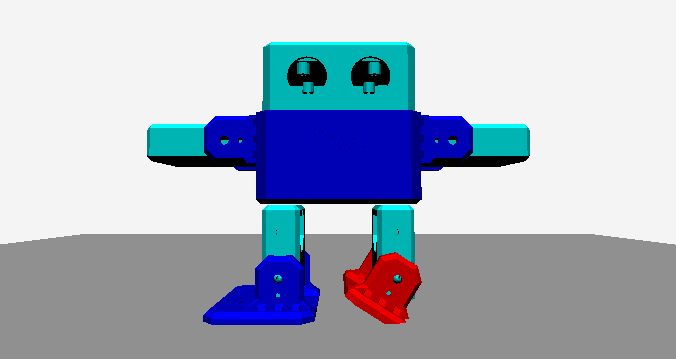
\includegraphics[width=0.4\textwidth]{images/otto-without-collision}}
\caption[Robot Otto - simulácia bez detekcie kolízií]{Robot Otto - simulácia bez detekcie kolízií}
\label{obr:otto-without-collision}
\end{figure}

\begin{figure}
\centerline{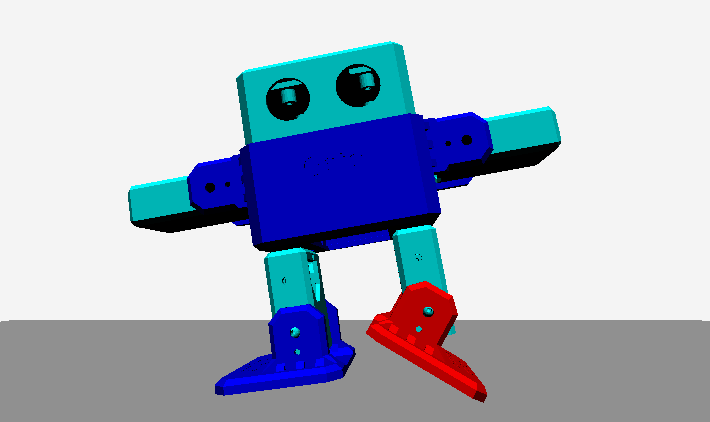
\includegraphics[width=0.4\textwidth]{images/otto-with-collision}}
\caption[Robot Otto - simulácia s detekciou kolízií]{Robot Otto - simulácia s detekciou kolízií}
\label{obr:otto-with-collision}
\end{figure}


%%%%%
% %%%    Riadiaci program robota
%%%%%
%\section{Riadiaci program robota}
%todo












